Para el circuito mostrado, obtenga

\begin{itemize}
  \item El valor DC de la corriente y el voltaje del diodo(punto de
  operación).
  \item El valor de $V_o$ en función de $V_i$.
\end{itemize}

\begin{figure}[H]
  \begin{center}
    \begin{circuitikz}

      \draw (0,0)
      to [sV, l=$v_i$] (0, 6)
      to [R, l=$100\Omega$] (2.5, 6)
      to [C, l=$C \to \infty$] (5, 6)
      to [D*, l_=$\mathrm{1N4148}$, i=$i_D$] (8, 6)
      to [R, l=$10\Omega$] (8, 3)
      to [battery, l=$25V$] (8, 0)
      to [short] (0, 0)
      ;

      \draw (5, 6)
      to [R, l=$24300\Omega$] (5, 0)
      ;

      \draw (8, 0)
      to [short] (16, 0)
      to [open, o-o, v=$v_o$] (16, 6)
      to [short] (14, 6)
      to [C, l_=$C \to \infty$] (11, 6)
      to [american controlled current source, l_=$10i_D$] (8, 6)
      ;

      \draw (11, 6)
      to [R, l=$1650\Omega$] (11,0)
      ;

      \draw (14, 6)
      to [R, l=$10k\Omega$] (14,0)
      ;
    \end{circuitikz}
  \end{center}
\end{figure}

\begin{figure}[H]
  \centering
  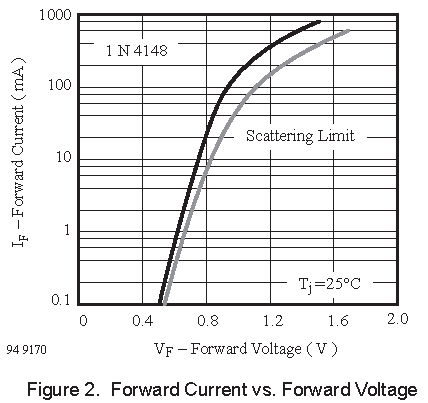
\includegraphics[width=0.5\textwidth]{1N4148}
\end{figure}

\newpage
\subsection{Solución}

Circuito en DC:
\begin{figure}[H]
  \begin{center}
    \begin{circuitikz}

      \draw (0, 0)
      to [R, l=$24300\Omega$] (0, 5)
      to [D*, l_=$\mathrm{1N4148}$, i_=$i_D$, v^<=$v_D$] (3, 5)
      to [R, l=$10\Omega$] (3, 2.5)
      to [battery, l=$25V$] (3, 0)
      to [short] (0, 0)
      ;

      \draw (3, 0)
      to [short] (6, 0)
      to [R, l=$1650\Omega$] (6, 5)
      to [american controlled current source, l_=$10i_D$] (3, 5)
      ;

    \end{circuitikz}
  \end{center}
\end{figure}

\begin{align*}
  24300 i_D + v_D  + 10 \cdot 11i_D &= 25\\
  1650 \cdot 10 i_D + 10 \cdot 11i_D &= 25 + v_i\\
  &\Rightarrow I_d = \frac{25-v_D}{24410}
\end{align*}

Si $v_D = 0.7V \Rightarrow i_D = \frac{243}{244100} \approx 995\mu A$

$995\mu A$ marca $\approx 0.6V$

\bigskip

Si $v_D = 0.6V \Rightarrow i_D = \frac{61}{61025} \approx 999.5\mu A$

$999.5\mu$ Marca $\approx 0.65V$

\bigskip

Se concluye que se tiene $i_D = 1mA$ y $v_D = 0.65V$, siendo estos
los valores del punto de operación. Así se tiene que $r_d = 25\Omega$.


\bigskip

Circuito en AC

\begin{figure}[H]
  \begin{center}
    \begin{circuitikz}

      \draw (0,0)
      to [sV, l=$v_i$] (0, 6)
      to [R, l=$100\Omega$] (2.5, 6)
      to [C, l=$C \to \infty$] (5, 6)
      to [D*, l_=$\mathrm{1N4148}$, i=$i_D$] (8, 6)
      to [R, l=$10\Omega$] (8, 3)
      to [battery, l=$25V$] (8, 0)
      to [short] (0, 0)
      ;

      \draw (5, 6)
      to [R, l=$24300\Omega$] (5, 0)
      ;

      \draw (8, 0)
      to [short] (16, 0)
      to [open, o-o, v=$v_o$] (16, 6)
      to [short] (14, 6)
      to [C, l_=$C \to \infty$] (11, 6)
      to [american controlled current source, l_=$10i_D$] (8, 6)
      ;

      \draw (11, 6)
      to [R, l=$1650\Omega$] (11,0)
      ;

      \draw (14, 6)
      to [R, l=$10k\Omega$] (14,0)
      ;
    \end{circuitikz}
  \end{center}
\end{figure}

*Parte b pendiente.
